% Options for packages loaded elsewhere
\PassOptionsToPackage{unicode}{hyperref}
\PassOptionsToPackage{hyphens}{url}
\documentclass[
  spanish,
  11pt,
]{article}
\usepackage{xcolor}
\usepackage[left=3cm,right=3cm,top=3cm,bottom=3cm]{geometry}
\usepackage{amsmath,amssymb}
\setcounter{secnumdepth}{-\maxdimen} % remove section numbering
\usepackage{iftex}
\ifPDFTeX
  \usepackage[T1]{fontenc}
  \usepackage[utf8]{inputenc}
  \usepackage{textcomp} % provide euro and other symbols
\else % if luatex or xetex
  \usepackage{unicode-math} % this also loads fontspec
  \defaultfontfeatures{Scale=MatchLowercase}
  \defaultfontfeatures[\rmfamily]{Ligatures=TeX,Scale=1}
\fi
\usepackage{lmodern}
\ifPDFTeX\else
  % xetex/luatex font selection
\fi
% Use upquote if available, for straight quotes in verbatim environments
\IfFileExists{upquote.sty}{\usepackage{upquote}}{}
\IfFileExists{microtype.sty}{% use microtype if available
  \usepackage[]{microtype}
  \UseMicrotypeSet[protrusion]{basicmath} % disable protrusion for tt fonts
}{}
\makeatletter
\@ifundefined{KOMAClassName}{% if non-KOMA class
  \IfFileExists{parskip.sty}{%
    \usepackage{parskip}
  }{% else
    \setlength{\parindent}{0pt}
    \setlength{\parskip}{6pt plus 2pt minus 1pt}}
}{% if KOMA class
  \KOMAoptions{parskip=half}}
\makeatother
\usepackage{graphicx}
\makeatletter
\newsavebox\pandoc@box
\newcommand*\pandocbounded[1]{% scales image to fit in text height/width
  \sbox\pandoc@box{#1}%
  \Gscale@div\@tempa{\textheight}{\dimexpr\ht\pandoc@box+\dp\pandoc@box\relax}%
  \Gscale@div\@tempb{\linewidth}{\wd\pandoc@box}%
  \ifdim\@tempb\p@<\@tempa\p@\let\@tempa\@tempb\fi% select the smaller of both
  \ifdim\@tempa\p@<\p@\scalebox{\@tempa}{\usebox\pandoc@box}%
  \else\usebox{\pandoc@box}%
  \fi%
}
% Set default figure placement to htbp
\def\fps@figure{htbp}
\makeatother
\ifLuaTeX
\usepackage[bidi=basic,shorthands=off]{babel}
\else
\usepackage[bidi=default,shorthands=off]{babel}
\fi
\ifLuaTeX
  \usepackage{selnolig} % disable illegal ligatures
\fi
\setlength{\emergencystretch}{3em} % prevent overfull lines
\providecommand{\tightlist}{%
  \setlength{\itemsep}{0pt}\setlength{\parskip}{0pt}}
\usepackage{caption}
\captionsetup[table]{position=bottom,labelformat=default,labelsep=colon,name=Tabla}
\captionsetup[figure]{labelformat=default,labelsep=colon,name=Figura}
\usepackage{booktabs}
\usepackage{longtable}
\usepackage{array}
\usepackage{multirow}
\usepackage{wrapfig}
\usepackage{float}
\usepackage{colortbl}
\usepackage{pdflscape}
\usepackage{tabularx}
\usepackage{xltabular}
\usepackage{threeparttable}
\usepackage{threeparttablex}
\usepackage[normalem]{ulem}
\usepackage{makecell}
\usepackage{xcolor}
\usepackage{bookmark}
\IfFileExists{xurl.sty}{\usepackage{xurl}}{} % add URL line breaks if available
\urlstyle{same}
\hypersetup{
  pdflang={es-ES},
  hidelinks,
  pdfcreator={LaTeX via pandoc}}

\author{}
\date{\vspace{-2.5em}}

\begin{document}

\begin{titlepage}
  \centering
  % Logo
  
\includegraphics[width=0.7\textwidth]{logo_facultad.png}\par
  % Espacio entre logo y título principal
  \vspace{3cm}
  % Título principal
  {\scshape\Huge Trabajo Práctico de Series de Tiempo \par}
  \vspace{1.5cm}
  % Subtítulo
  {\itshape\LARGE Análisis de muertes por Accidentes Cerebrovasculares (ACV) en Estados Unidos \par}
  % Esto llena todo el espacio intermedio
  \vfill
  % Carrera y Alumna, cerca de la fecha
  {\Large Alumna: Cañizares, Maria Ines \par}
  \vspace{0.5cm}
  {\Large Licenciatura en Estadística \par}
  % Fecha abajo del todo
  \vspace{1cm}
  {\large Año 2026 \par}
\end{titlepage}

\begin{verbatim}
## # A tsibble: 264 x 2 [1M]
##        Month muertes
##        <mth>   <int>
##  1 1999 ene.   16628
##  2 1999 feb.   14728
##  3 1999 mar.   16197
##  4 1999 abr.   13983
##  5 1999 may.   13246
##  6 1999 jun.   12395
##  7 1999 jul.   12453
##  8 1999 ago.   12566
##  9 1999 sep.   12493
## 10 1999 oct.   13691
## # i 254 more rows
\end{verbatim}

\begin{figure}

{\centering 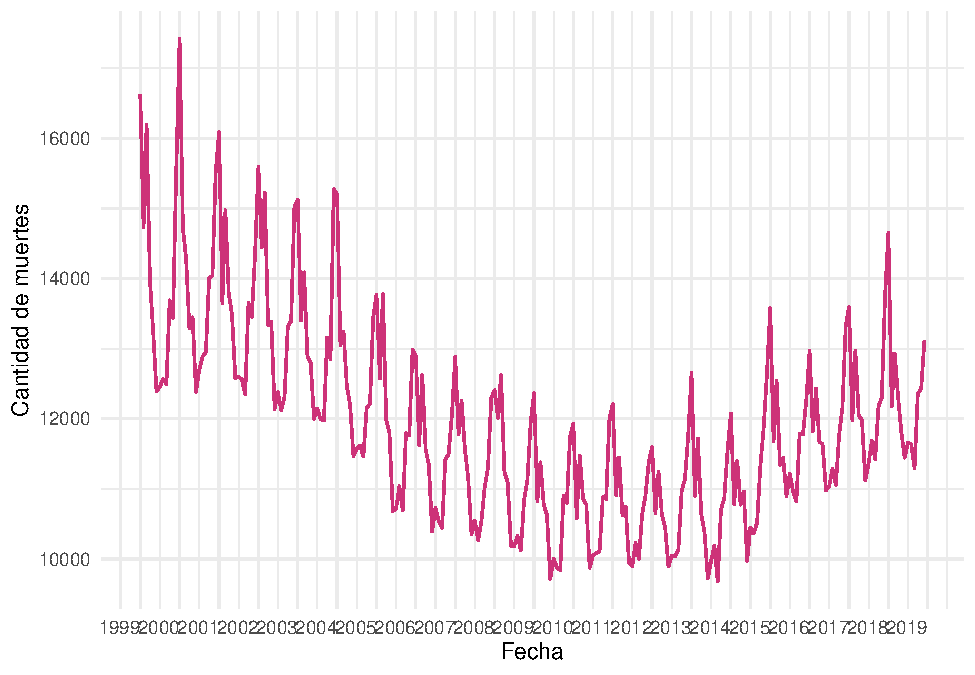
\includegraphics[width=0.7\linewidth,height=0.7\textheight]{TP---M-Ines-Cañizares_files/figure-latex/unnamed-chunk-2-1} 

}

\caption{Evolución de las muertes mensuales por ACV en Estados Unidos (1999–2018)}\label{fig:unnamed-chunk-2}
\end{figure}

\begin{figure}

{\centering 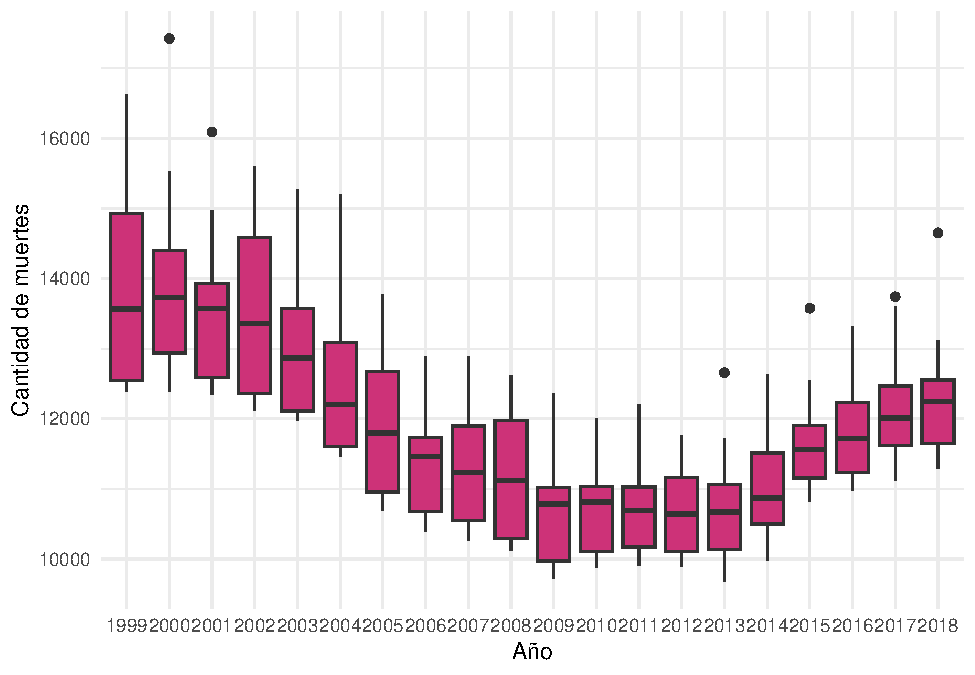
\includegraphics[width=0.7\linewidth,height=0.7\textheight]{TP---M-Ines-Cañizares_files/figure-latex/unnamed-chunk-3-1} 

}

\caption{Distribución Anual de Muertes por ACV en EE.UU. (1999–2018)}\label{fig:unnamed-chunk-3}
\end{figure}

\begin{figure}

{\centering 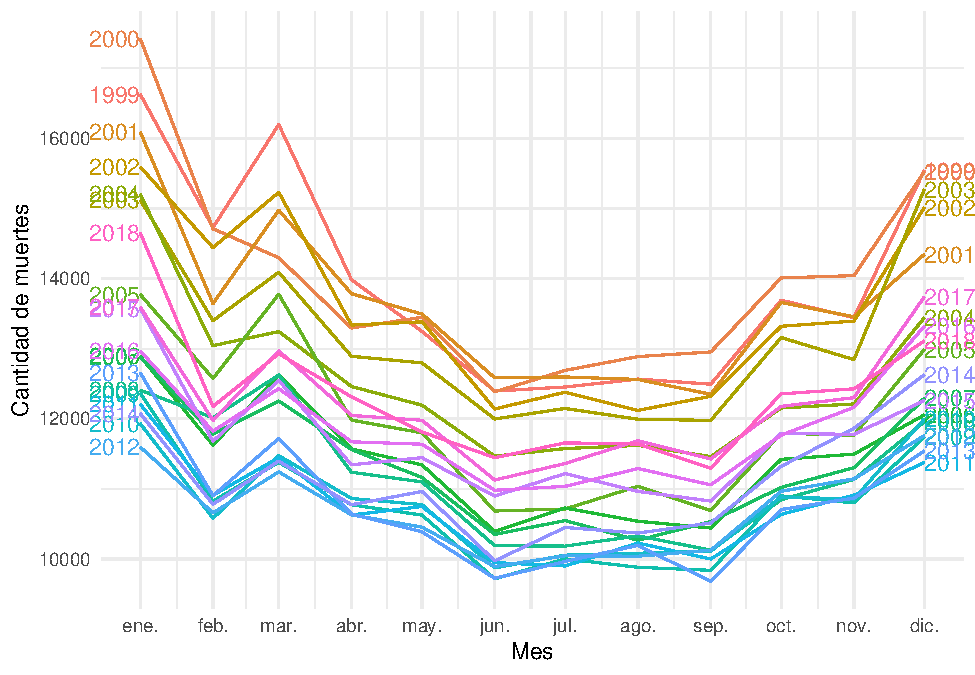
\includegraphics[width=0.7\linewidth,height=0.7\textheight]{TP---M-Ines-Cañizares_files/figure-latex/unnamed-chunk-4-1} 

}

\caption{Gráfico estacional de Muertes por ACV en EE.UU. (1999–2018)}\label{fig:unnamed-chunk-4}
\end{figure}

\begin{figure}

{\centering 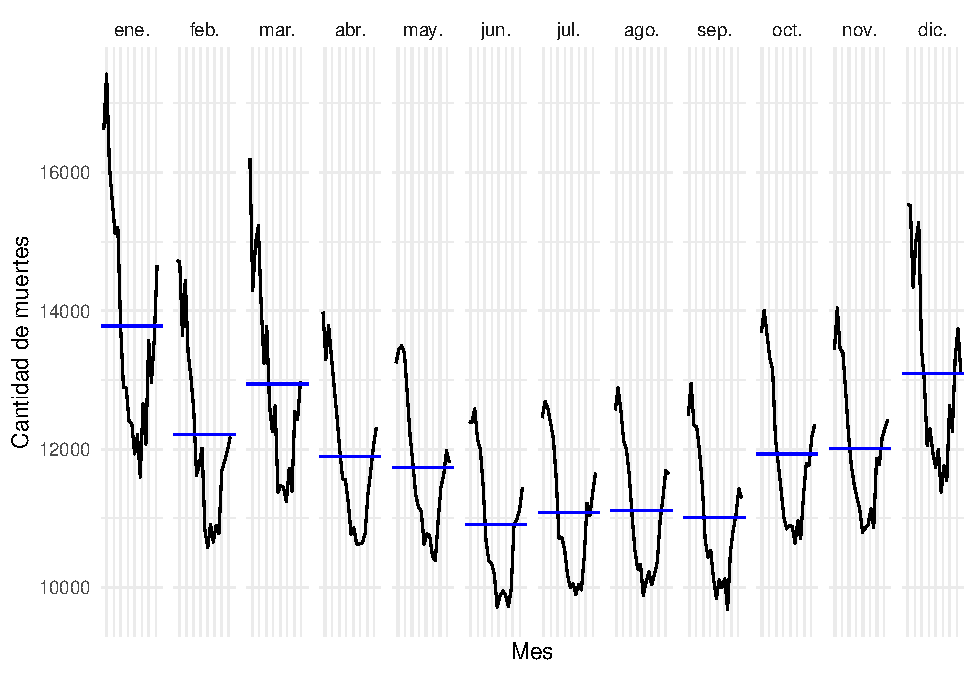
\includegraphics[width=0.7\linewidth,height=0.7\textheight]{TP---M-Ines-Cañizares_files/figure-latex/unnamed-chunk-5-1} 

}

\caption{Gráfico de subseries estacionales de muertes por ACV en EE.UU. (1999-2018)}\label{fig:unnamed-chunk-5}
\end{figure}

\begin{figure}

{\centering 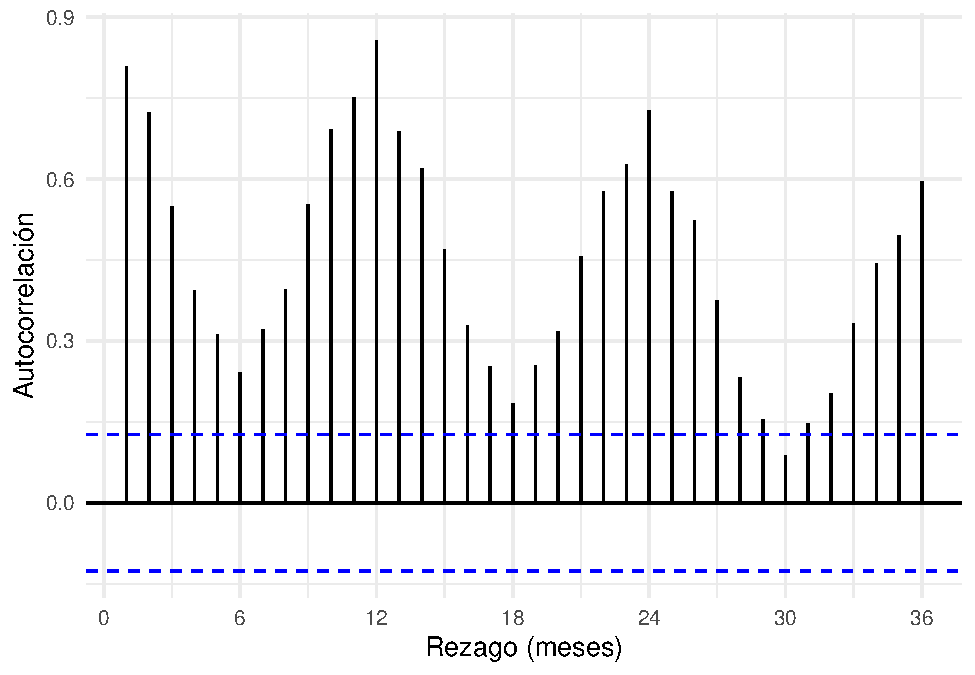
\includegraphics[width=0.7\linewidth,height=0.7\textheight]{TP---M-Ines-Cañizares_files/figure-latex/unnamed-chunk-6-1} 

}

\caption{Función de Autocorrelación de las Muertes por ACV}\label{fig:unnamed-chunk-6}
\end{figure}

\end{document}
